 \documentclass[conference]{IEEEtran}
\IEEEoverridecommandlockouts

\usepackage{cite}
\usepackage{amsmath,amssymb,amsfonts}
\usepackage{graphicx}
\usepackage{textcomp}
\usepackage{xcolor}
\usepackage{booktabs}
\usepackage{array}
\usepackage{url}

\def\BibTeX{{\rm B\kern-.05em{\sc i\kern-.025em b}\kern-.08em
    T\kern-.1667em\lower.7ex\hbox{E}\kern-.125emX}}

\begin{document}

\title{Detection of Coordinated Social Media Behavior with Large Language Models and Multi-Layer Account Graphs}

\author{
\IEEEauthorblockN{Tsung-Yuan Lin}
\IEEEauthorblockA{\textit{Department of Information Engineering and} \\
\textit{Computer Science} \\
\textit{Feng Chia University}\\
Taichung, Taiwan \\
D1285270@o365.fcu.edu.tw}
\and
\IEEEauthorblockN{Jyun-Hao Chang}
\IEEEauthorblockA{\textit{Department of Information Engineering and} \\
\textit{Computer Science} \\
\textit{Feng Chia University}\\
Taichung, Taiwan \\
D1285182@o365.fcu.edu.tw}
\and
\IEEEauthorblockN{Jia-An Lai}
\IEEEauthorblockA{\textit{Department of Information Engineering and} \\
\textit{Computer Science} \\
\textit{Feng Chia University}\\
Taichung, Taiwan \\
D1285223@o365.fcu.edu.tw}
\and
\IEEEauthorblockN{Chiung-Hon Lee}
\IEEEauthorblockA{\textit{Department of Information Engineering and} \\
\textit{Computer Science} \\
\textit{Feng Chia University}\\
Taichung, Taiwan \\
cholee@o365.fcu.edu.tw}
}

\maketitle

\begin{abstract}
Suspicious information operations on social media may appear not only as abnormal individual accounts, but also as shared targets, similar stances, and temporally close actions among multiple accounts. In practice, analysts need tools that can organize suspicious evidence and prioritize cases for review, similar to how plagiarism-screening systems highlight suspicious passages without deciding misconduct by themselves. This paper proposes Manipulative and Coordinated Account (MCA) Detector, an evidence-assisted review pipeline for discovering candidate coordinated groups in Reddit Bitcoin discussions. The system combines large language model (LLM)-based stance analysis, multi-layer account graphs, MCA seed ranking, candidate group expansion, and temporal synchronization verification. MCA Detector outputs candidate groups, account rankings, intra-group relations, and temporal evidence to support human interpretation.
\end{abstract}

\begin{IEEEkeywords}
social media analysis, coordinated behavior detection, large language models, multi-layer graph analysis, temporal synchronization
\end{IEEEkeywords}

\section{Introduction}
Social media has become an important space for the circulation of financial information and the formation of investor sentiment. In Bitcoin-related communities, price fluctuations and market news often trigger large volumes of discussion within a short period. This environment also allows influence behavior to appear as group-level patterns: several accounts may repeatedly criticize the same targets, use inflammatory rhetoric, or enter the same discussion threads within close time intervals. Such behavior is difficult to inspect manually because the relevant evidence is scattered across text, account activity, interaction targets, and timestamps.

Many previous studies have focused on whether an individual account exhibits bot-like or anomalous characteristics, such as posting frequency or content repetition. However, coordinated influence is often a group-level review problem rather than a single-account classification problem. Multiple accounts may share targets because they are genuinely coordinated, but they may also do so because they participate in the same community and hold similar viewpoints. Therefore, a practical system should not only rank suspicious accounts, but also expose the group-level relations and temporal evidence behind that ranking.

To address this problem, this paper proposes Manipulative and Coordinated Account (MCA) Detector, an evidence-assisted review pipeline for detecting candidate coordinated behavior in social media, using the Bitcoin subreddit on Reddit as the experimental setting. In this work, the MCA score is an account-level review priority indicator. It measures candidate risk across manipulative content, coordination signals, interaction influence, and behavioral anomaly dimensions, and then uses high-priority accounts as seeds for group-level evidence discovery.

The intended users include platform moderators, community managers, threat intelligence analysts, researchers, journalists, and public-interest organizations that need to inspect suspicious group-level behavior from publicly observable social media data. For these users, MCA Detector is designed to reduce the cost of initial triage by converting scattered posts, comments, account relations, and timestamps into reviewable evidence.

The main work of this paper is summarized as follows:
\begin{itemize}
    \item We propose an evidence-assisted review pipeline that converts large-scale discussion data into candidate groups and interpretable evidence tables.
    \item We integrate large language models and multi-layer account graphs to transform textual semantics into analyzable interaction and structural signals.
    \item We combine candidate group expansion with temporal synchronization verification to separate shared-target structure from stronger timing-based review evidence.
\end{itemize}

The remainder of this paper is organized as follows. Section II reviews
related work from three perspectives: account-level bot and anomaly
detection, graph-based coordinated behavior detection, and stance analysis on
social platforms. Section III presents the system design, including LLM-based
semantic analysis, multi-layer graph construction with MCA seed ranking, and
the two-stage process of group expansion and temporal verification. Section
IV reports the experimental setting, candidate group outputs, temporal
baseline comparison, and two contrasting case studies. Section V discusses
system interpretation and scope, and Section VI concludes the paper.

\section{Related Work}
\subsection{Social Bots and Account Anomaly Detection}
Early research on abnormal social media behavior mainly focused on bot detection at the individual account level. Ferrara et al. discussed how social bots can affect online ecosystems through automated content generation, social network interaction, and persuasive or deceptive behavior \cite{b1}. Varol et al. further built a Twitter bot detection framework using a wide range of features, including account metadata, content, sentiment, network patterns, and activity time series \cite{b2}. These studies show that account-level features are useful for identifying automation or abnormal behavior.

However, account-level bot detection is not the same as coordinated behavior detection. A highly active human user may appear abnormal, while a manually operated account may still participate in coordinated manipulation. In cryptocurrency communities, this distinction is especially important because users may naturally post frequently, react quickly to market news, or express strong opinions. Therefore, this paper uses account-level anomaly and influence features as seed-ranking signals that guide later group-level evidence collection.

\subsection{Coordinated Behavior Detection and Graph Analysis}
Compared with single-account detection, coordinated behavior detection focuses on whether multiple accounts exhibit similar or synchronized behavioral patterns. Cresci et al. proposed Social Fingerprinting, which models account behavior as digital DNA sequences and detects groups of spambots through behavioral similarity \cite{b3}. Mazza et al. focused on temporal patterns in retweet behavior and used these patterns to identify suspicious botnets \cite{b4}. These studies suggest that coordination is often clearer at the group level than at the individual-account level.

More recent work has further developed coordination network approaches. Pacheco et al. constructed coordination networks from shared behavioral traces, such as identities, images, hashtags, retweets, and temporal patterns, and applied the method to several influence-campaign cases, including cryptocurrency-related manipulation \cite{b5}. Graham et al. proposed the Coordination Network Toolkit, which represents different types of coordinated behavior using weighted directed multigraphs \cite{b6}. These studies show that coordination can be represented as graph structure, but the specific traces depend on the platform being analyzed.

\subsection{Stance Analysis and Reddit-specific Detection}
Coordinated behavior in social media is not only reflected in interaction structures, but may also appear in textual stance and rhetorical style. Mohammad et al. formulated stance detection as identifying whether a text supports, opposes, or is neutral toward a specific target \cite{b7}. This idea is useful for Reddit because comments are often direct responses to a post author or a discussion target. Language models are useful in this setting because stance, tone, and implicit rhetorical cues are difficult to capture with keyword or frequency-based features alone.

Reddit-specific malicious-account studies also show that suspicious actors may not behave like simple bots. Saeed et al. proposed TROLLMAGNIFIER, a system trained on known Russian-sponsored troll accounts on Reddit, and showed that troll accounts can display loose coordination, topic similarity, and temporal synchronization \cite{b8}. Their work is based on known labeled troll accounts. Our project instead studies an unlabeled review setting, where the system must surface candidate groups and explain the evidence available for inspection.

\subsection{Position of This Work}
Overall, prior work provides three important lessons. First, bot and anomaly detection can help identify accounts that deserve attention. Second, graph-based coordination methods can reveal shared targets and synchronized behaviors, but a single graph layer may be affected by popular topics or natural interactions among users with similar viewpoints. Third, stance analysis can connect textual meaning with account relations. MCA Detector combines these ideas by adapting coordination networks to Reddit replies: comment stance is converted into signed account-to-account relations, multi-layer graphs are used for candidate discovery, and temporal synchronization is used as separate review evidence.

\begin{figure}[htbp]
\centering
\includegraphics[width=0.95\linewidth]{fig1_pipeline.png}
\caption{MCA Detector analysis pipeline.}
\label{fig:pipeline}
\end{figure}

\section{Methodology and System Architecture}
\subsection{Overall Pipeline}
MCA Detector is an analysis pipeline centered on high-risk candidate coordination group discovery and reviewable evidence generation. It identifies candidate groups from large-scale social media data and provides multi-layer evidence, including content, behavior, account relations, and temporal synchronization, for subsequent human review.

Fig.~\ref{fig:pipeline} summarizes the overall workflow. The pipeline begins with social media data. LLM-based stance analysis is first applied to extract post rhetoric and comment stance signals. Multi-layer account graphs are then constructed from account interactions. Next, accounts are ranked by their MCA scores to select candidate seed accounts for review. Stage 1 expands each seed account into a candidate group by identifying accounts with shared interaction targets or similar structural signals. Stage 2 performs temporal synchronization verification by examining whether accounts within a candidate group appear in the same discussion thread within short time intervals. Finally, the system outputs candidate coordination group summaries, account-level review rankings, intra-group relations, and temporal synchronization evidence for human interpretation.

The generated artifacts are intended to be inspected through an evidence
viewer. Fig.~\ref{fig:demo-placeholder} reserves space for the demo website
screenshot, and Table~\ref{tab:outputs} summarizes the main outputs shown to
reviewers.

\begin{figure*}[htbp]
\centering
\begin{tabular}{cc}
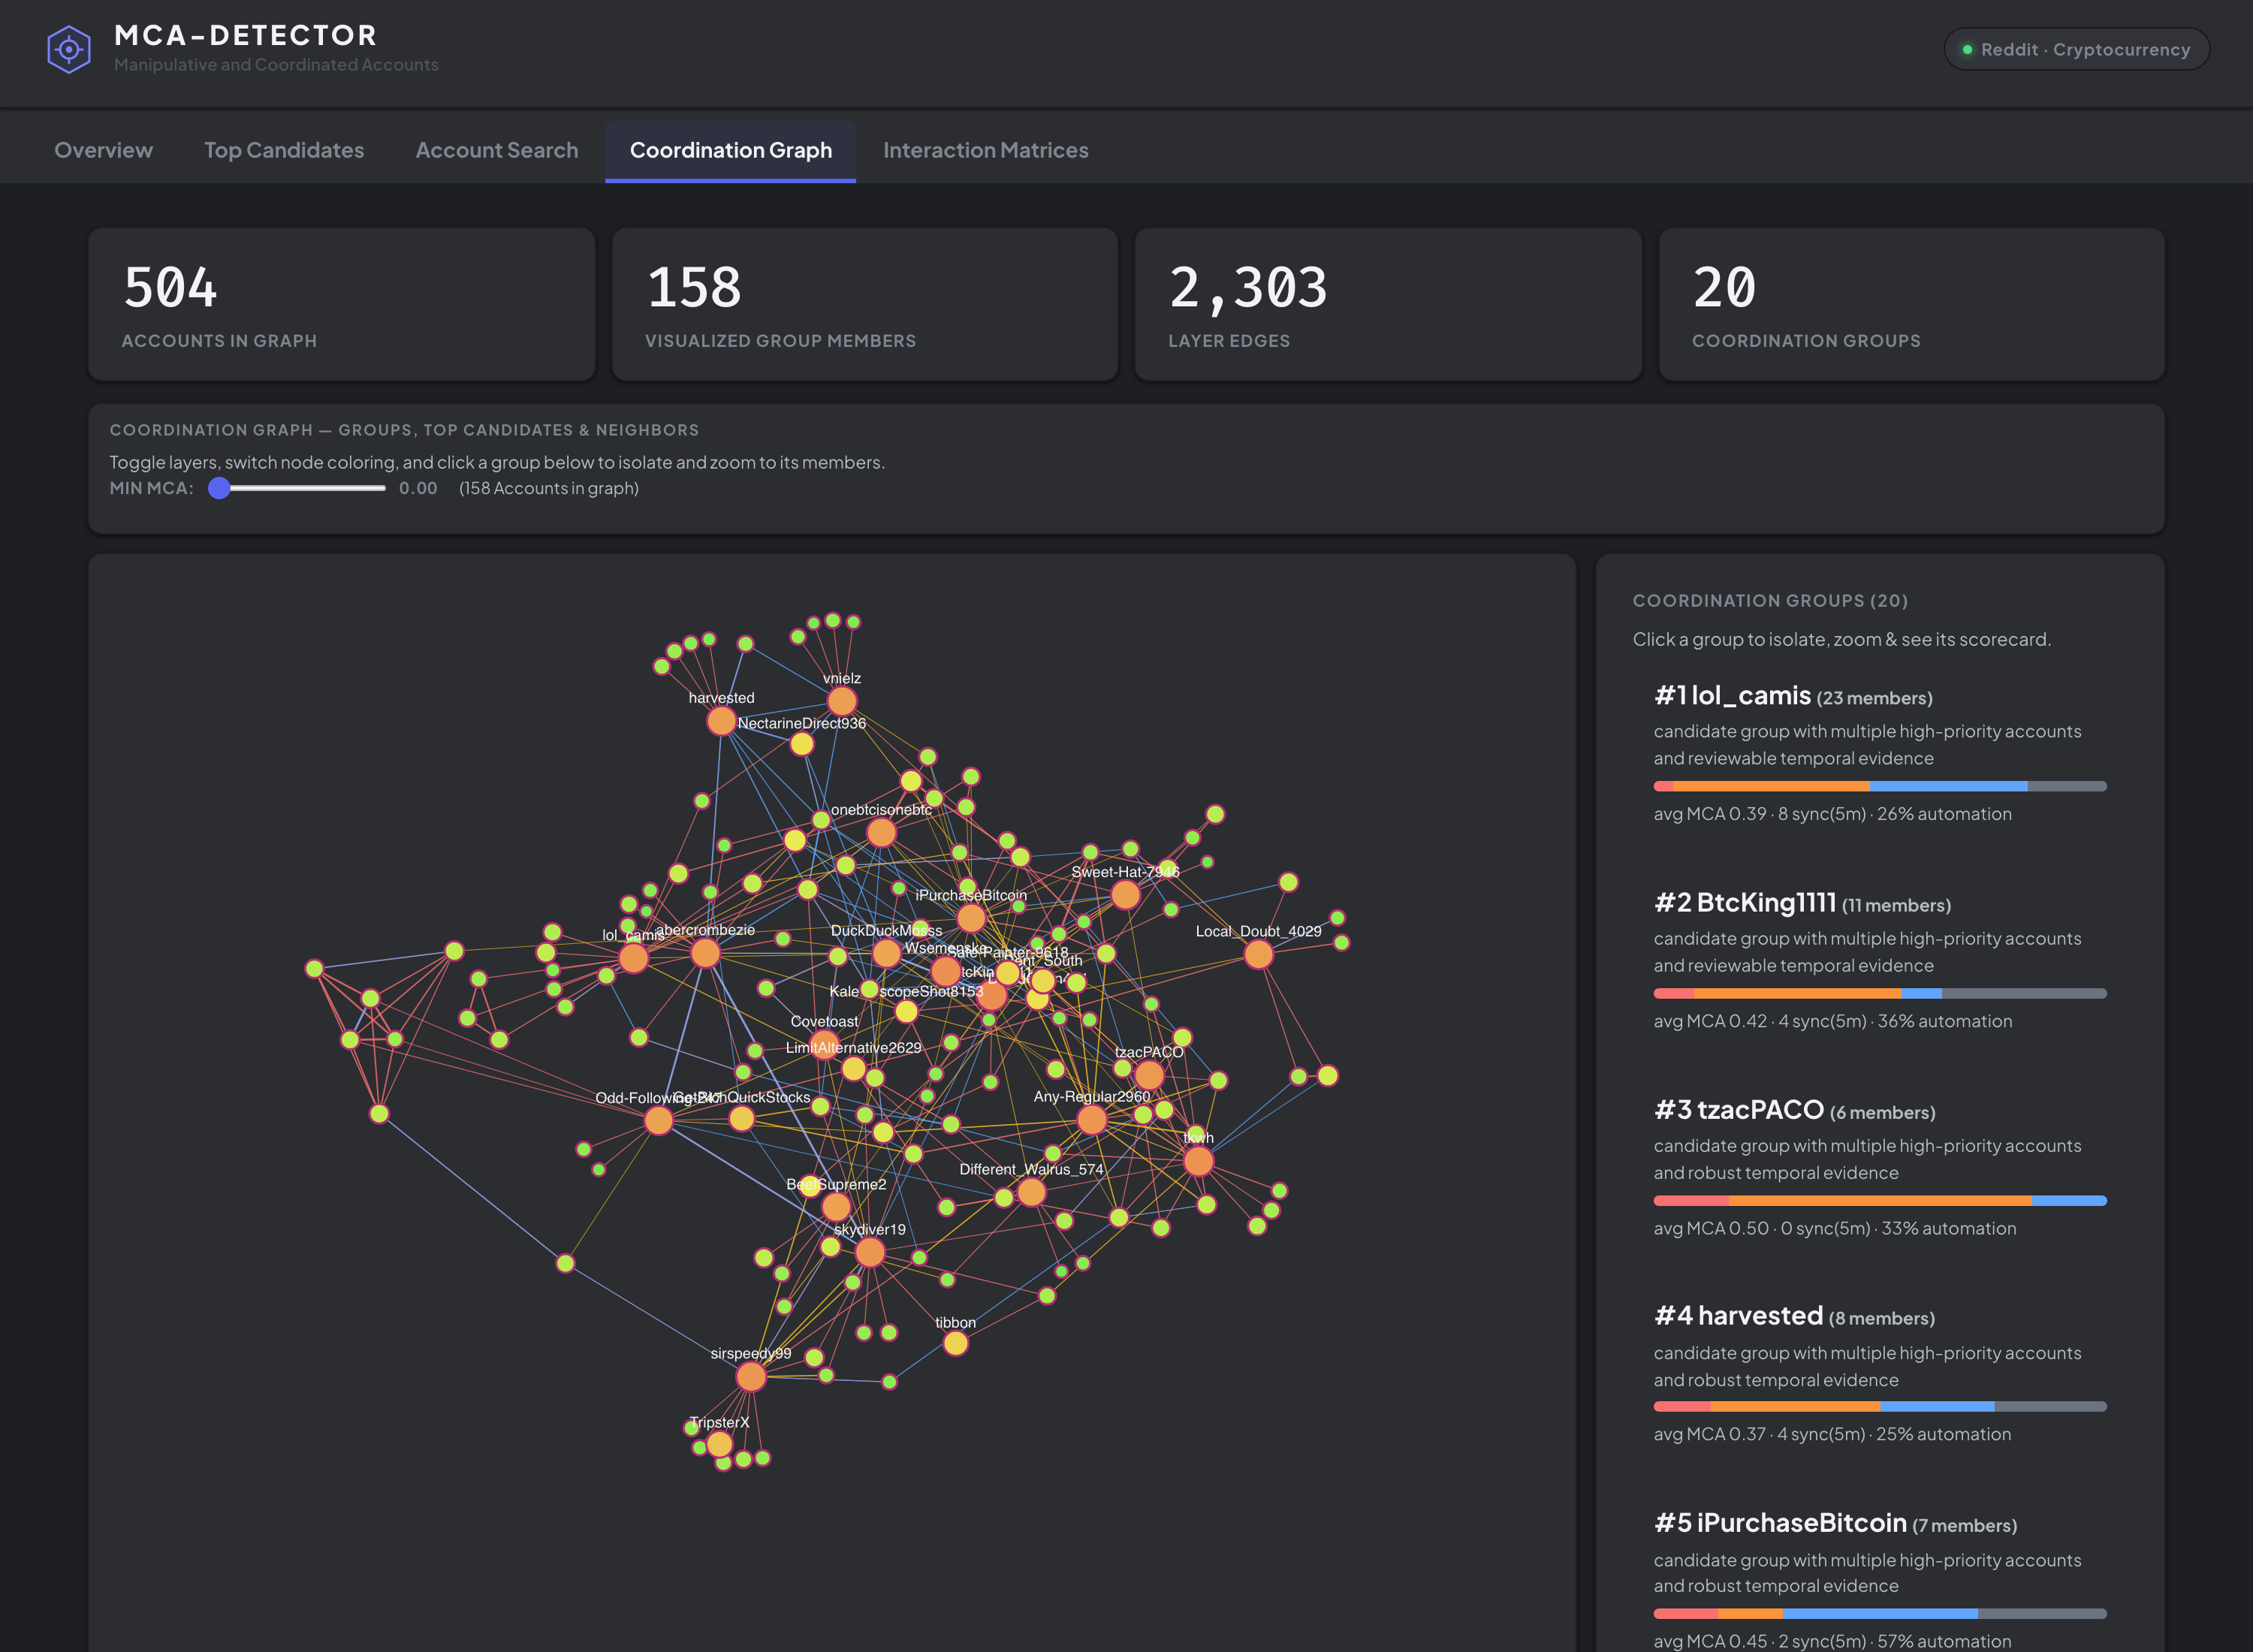
\includegraphics[width=0.48\textwidth]{final-a.png} &
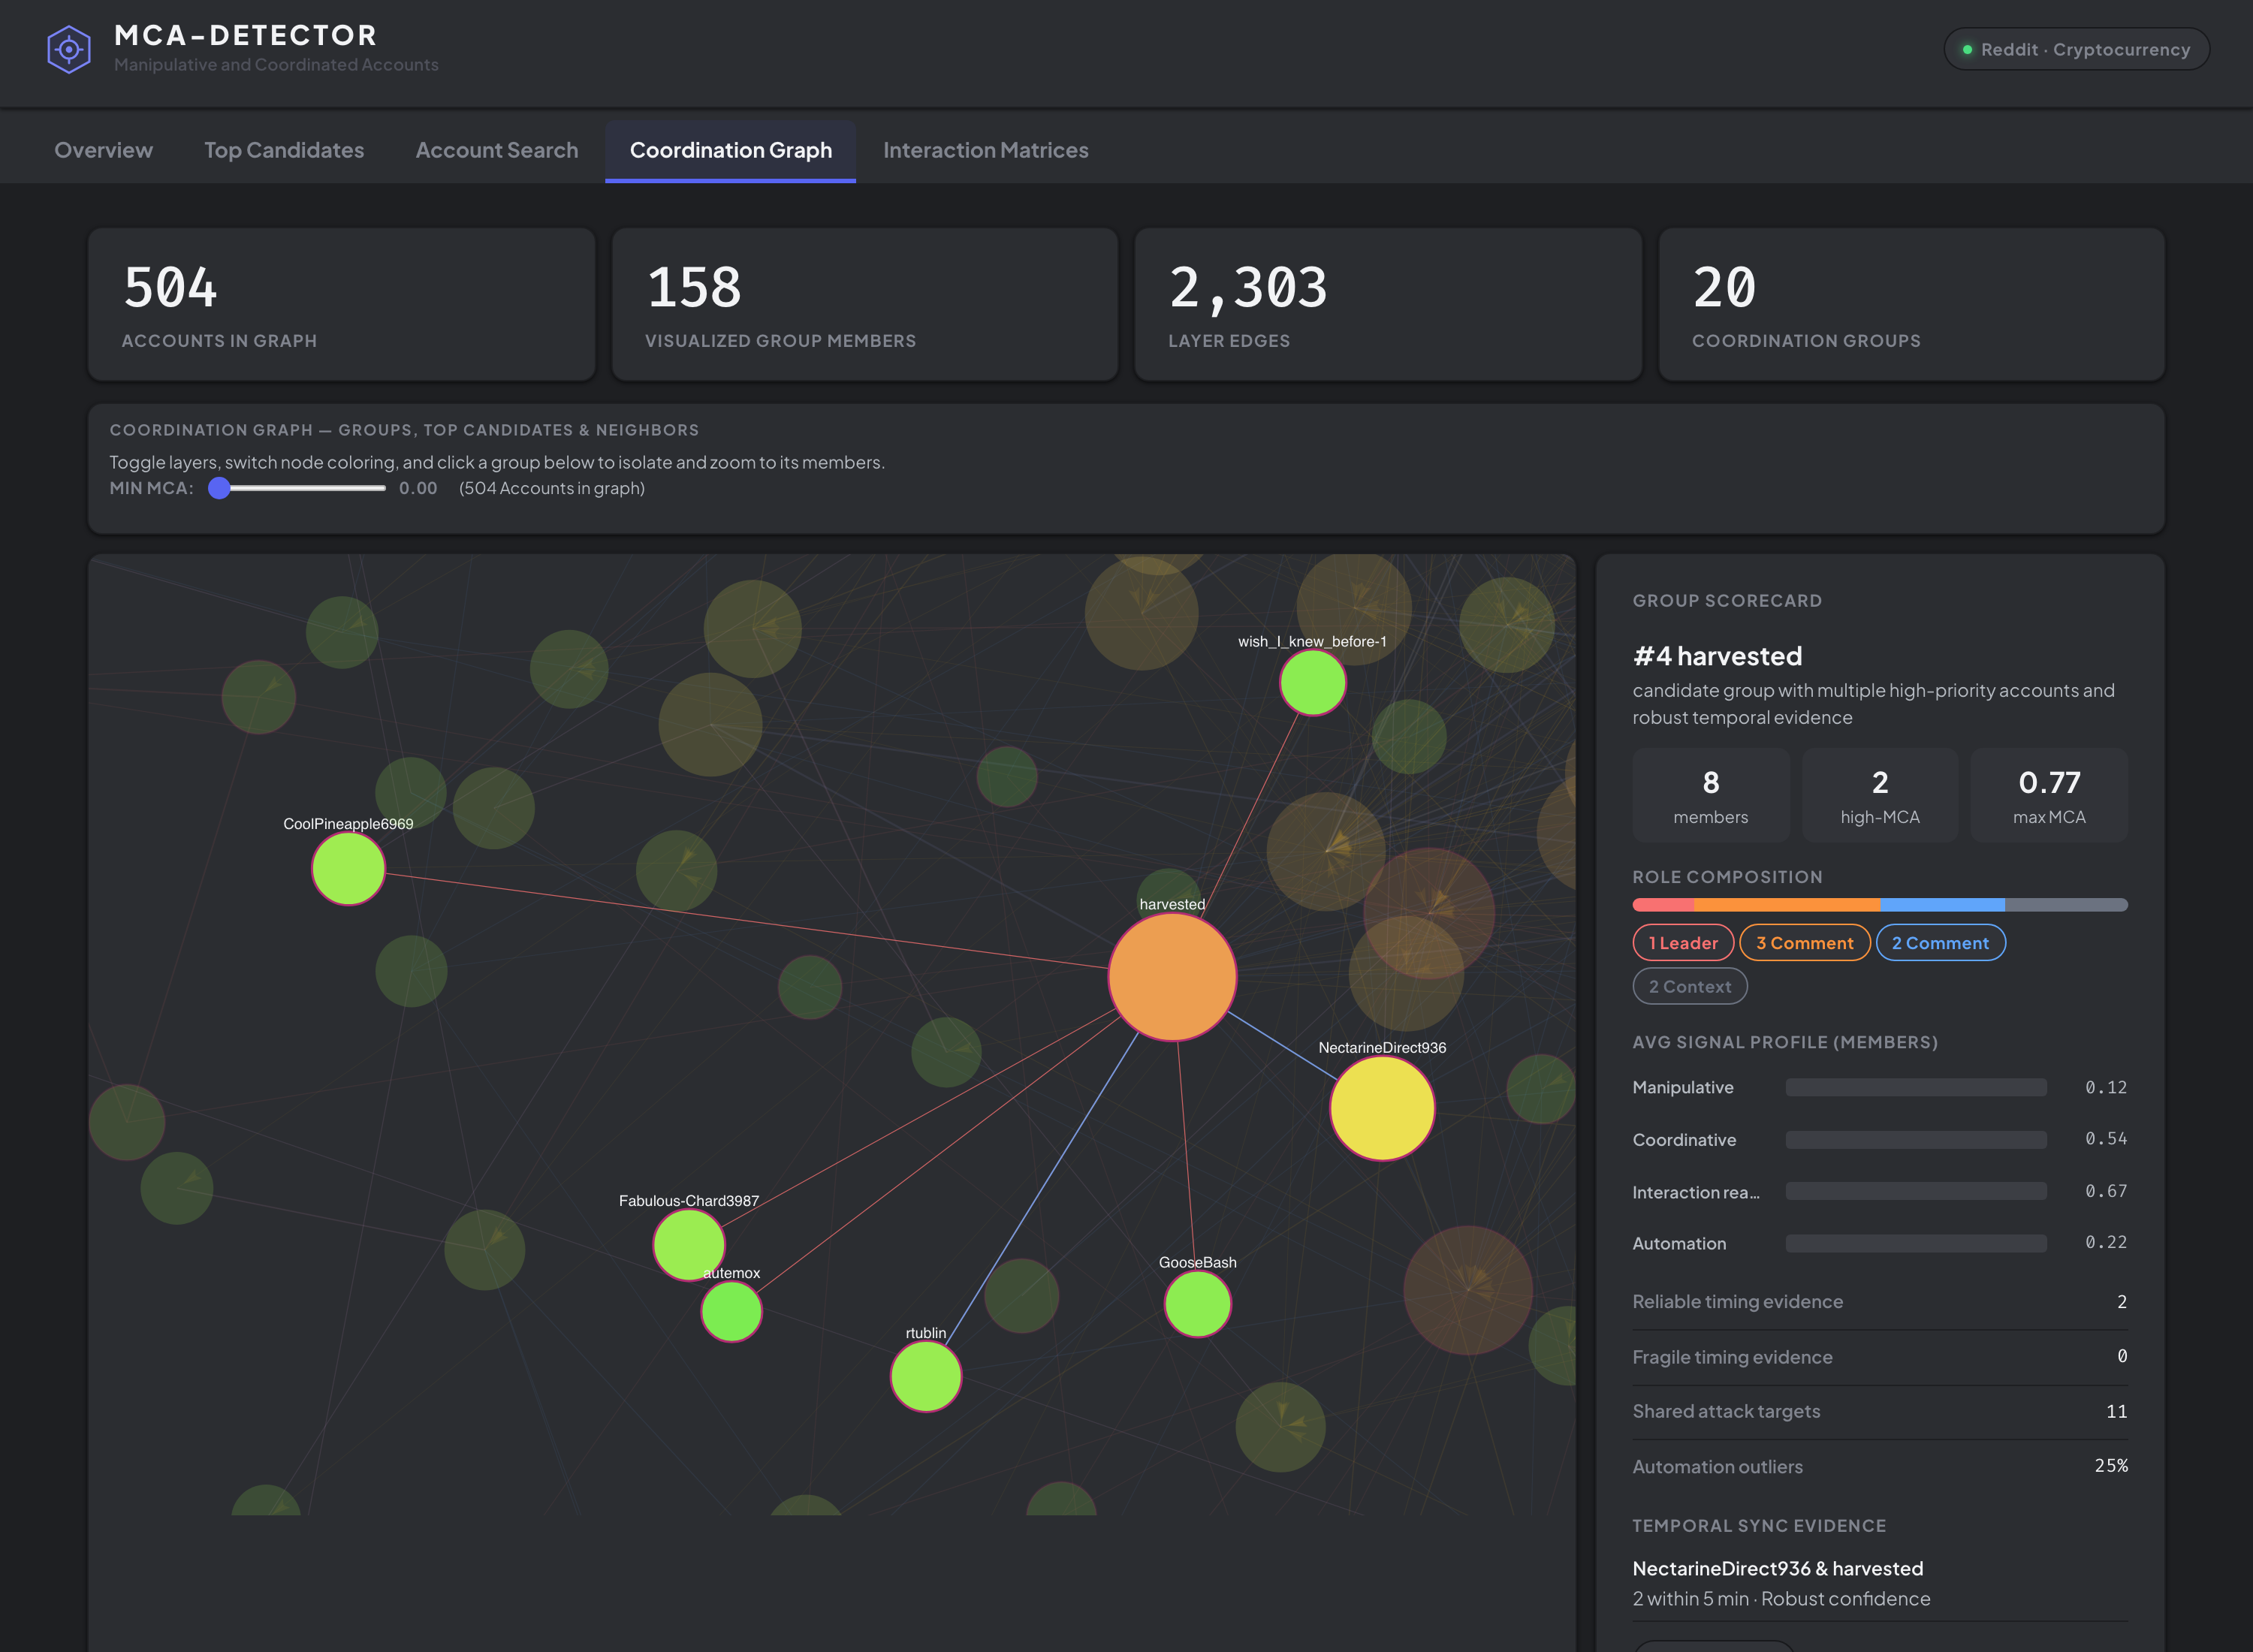
\includegraphics[width=0.48\textwidth]{final-b.png} \\
(a) Candidate group triage view & (b) Selected group evidence view
\end{tabular}
\caption{Demo evidence viewer showing graph-level triage and selected group evidence. The dashboard visualizes a subset of generated artifacts for inspection; aggregate experimental statistics are reported separately in Table~\ref{tab:results}.}
\label{fig:demo-placeholder}
\end{figure*}

\begin{table}[htbp]
\caption{Main Output Artifacts of MCA Detector}
\label{tab:outputs}
\centering
\begin{tabular}{p{0.34\linewidth}p{0.56\linewidth}}
\toprule
\textbf{Output} & \textbf{Purpose} \\
\midrule
Account ranking & Lists high-priority MCA seed accounts. \\
Candidate groups & Shows expanded members and inclusion reasons. \\
Pair evidence & Records same-thread timing and temporal confidence. \\
Role table & Labels simple group roles such as attacker, supporter, and leader-instigator. \\
Demo dashboard & Visualizes group ranking and evidence for review. \\
\bottomrule
\end{tabular}
\end{table}

\subsection{LLM-based Semantic Analysis and Account Relation Construction}
The system uses large language models to analyze Reddit posts and comments. The motivation is to capture stance, tone, and implicit rhetorical cues that are difficult to represent using simple keyword matching or word-frequency features. For posts, the model outputs a sentiment score, a manipulative rhetoric score, and rhetoric labels that describe whether the post contains fear appeals, urgency, appeals to authority, group polarization, or calls to action. For comments, the model identifies the stance of each comment toward the original post author, including support, opposition, neutrality, mixed stance, and unclear stance.

The results of comment stance analysis are converted into account-level interaction relations. If account $A$ comments under a post written by account $B$, a directed interaction edge from $A$ to $B$ is created. If the comment expresses support, the edge is treated as a positive interaction. If the comment expresses opposition or attack, the edge is treated as a negative interaction. Through this process, unstructured text is transformed into account interaction edges for subsequent graph analysis.

\subsection{Multi-layer Graphs and MCA Seed Ranking}
After semantic analysis, the system constructs multi-layer account graphs, including a basic interaction graph, positive and negative interaction graphs, a shared negative target graph, a triggered response graph, and a rhetoric label similarity graph. Among these layers, the shared negative target graph measures whether two accounts frequently oppose the same set of targets. It serves as the main signal for candidate group discovery because shared negative targets directly capture repeated pressure toward similar accounts.

Each graph layer captures a different type of evidence and also has its own failure mode. The basic interaction graph may be strongly affected by highly active accounts. The shared target graph may become broad when many users comment on the same popular authors. The rhetoric similarity graph can reflect similar topics or writing styles. For this reason, MCA Detector does not rely on a single graph layer. Instead, the shared negative target graph is used as the main discovery signal, while other graph layers provide supporting evidence and review context.

The MCA score integrates four categories of signals: manipulative content, coordination clues, interaction influence, and behavioral anomaly. It estimates the review priority of an account as a candidate seed for later group expansion.

\begin{equation}
S_{MCA}=0.30S_M+0.35S_C+0.15S_I+0.20S_A,
\end{equation}
where $S_M$, $S_C$, $S_I$, and $S_A$ denote manipulative content, coordination clues, interaction influence, and behavioral anomaly, respectively. These weights are interpretable review weights rather than supervised parameters.

Table~\ref{tab:mca-score} summarizes the four signal categories used by the
MCA score.

\begin{table}[htbp]
\caption{Signal Categories Used in the MCA Score}
\label{tab:mca-score}
\centering
\begin{tabular}{p{0.27\linewidth} p{0.62\linewidth}}
\toprule
\textbf{Signal category} & \textbf{Main content} \\
\midrule
Manipulative content & Average manipulative rhetoric score, non-neutral rhetoric ratio, opposition stance ratio \\
Coordination clues & Shared targets, shared negative targets, triggered response frequency \\
Interaction influence & Active comment volume, reply volume, interaction breadth \\
Behavioral anomaly & Isolation Forest anomaly score derived from activity frequency, burstiness, and time-of-day distribution \\
\bottomrule
\end{tabular}
\end{table}

\subsection{Candidate Group Expansion and Temporal Synchronization Verification}
This paper uses a two-stage process to discover candidate coordinated groups. Stage 1 begins with high-scoring MCA seed accounts and expands candidate groups in a layered manner. Accounts whose shared negative target weights exceed a threshold can be directly included. Rhetoric label similarity and triggered response relations are used as auxiliary signals and require additional structural support before inclusion. The system also searches outward from already included members to find indirectly related accounts. To avoid excessive group expansion, a new candidate account must have shared negative target relations with at least two existing group members.

The expansion rules are designed to keep the candidate groups reviewable. If the system expands groups only by loose shared targets, the candidate group may become too large and difficult to inspect manually. Therefore, accounts with strong shared negative target relations can be included directly, while weaker signals such as rhetoric similarity or triggered response relations require additional structural support. For indirect expansion, a new account must be connected to at least two existing members through shared negative target relations. This rule helps prevent candidate groups from growing only because of one weak connection.

A lightweight threshold sensitivity check was also conducted. When the co-negative-target threshold was set to 0.10 and 0.20, the pipeline produced the same 172 unique candidate accounts and the same 13 strong, 8 moderate, and 3 robust temporal pairs under the current top-neighbor cap. Increasing the threshold to 0.30 reduced the candidate set to 55 accounts and retained 4 strong, 0 moderate, and 2 robust temporal pairs.

Stage 2 verifies temporal synchronization for all account pairs within each candidate group. The system checks whether two accounts appear in the same post or discussion thread and calculates whether the time difference between their comments falls within 5 or 30 minutes. If a pair appears within 5 minutes, it is marked as strong temporal synchronization. If the pair appears multiple times within 30 minutes or appears within short intervals across multiple posts, it is marked as moderate temporal synchronization. The system further assigns temporal confidence levels, including robust, moderate-review, and fragile evidence, to avoid over-interpreting accidental co-occurrence.

Temporal strength and temporal confidence are separated because they describe different aspects of evidence. A strong temporal synchronization label means that at least one very short time-window event exists. However, if this evidence appears only once in a popular thread, it may still be a coincidence. Temporal confidence is therefore used to describe whether the timing evidence is repeated or stable enough for review. In other words, strong synchronization indicates a short time gap, while robust confidence indicates more reliable temporal evidence.

\section{Experimental Design and Results}
\subsection{Evaluation Setting}
Because this study does not use a large manually labeled dataset of confirmed coordinated and non-coordinated accounts, the experiment does not report precision, recall, F1-score, or classification accuracy. Instead, the evaluation focuses on an evidence-assisted review question: whether the pipeline can reduce a large number of accounts into a smaller set of candidate groups and provide interpretable evidence for each group.

\subsection{Candidate Groups and Temporal Synchronization Results}
The experimental results show that MCA Detector can reduce a large set of accounts into a smaller candidate range suitable for inspection. As shown in Table~\ref{tab:results}, the system selected 20 seed accounts based on MCA scores and generated 20 candidate groups after group expansion. After removing duplicates, the system identified 172 unique candidate accounts. Stage 2 temporal synchronization verification further found 13 strong temporal synchronization pairs and 8 moderate temporal synchronization pairs, among which 3 pairs reached robust temporal confidence.

\begin{table}[htbp]
\caption{Summary of Candidate Groups and Temporal Synchronization Results}
\label{tab:results}
\centering
\begin{tabular}{lc}
\toprule
\textbf{Metric} & \textbf{Value} \\
\midrule
Selected seed accounts & 20 \\
Candidate seed groups & 20 \\
Unique candidate accounts & 172 \\
Strong temporal sync pairs & 13 \\
Moderate temporal sync pairs & 8 \\
Robust temporal pairs & 3 \\
Moderate-review temporal pairs & 44 \\
\bottomrule
\end{tabular}
\end{table}

To check whether temporal evidence only reflects high activity, we compared candidate pairs with random active pairs and activity-controlled random pairs sampled from similar comment-count bins. Candidate pairs show higher same-post overlap and higher temporal evidence rates than both baselines, as shown in Table~\ref{tab:temporal-baseline}.

\begin{table}[htbp]
\caption{Temporal Baseline Comparison}
\label{tab:temporal-baseline}
\centering
\begin{tabular}{lcccc}
\toprule
\textbf{Pair set} & \textbf{Same-post} & \textbf{Strong} & \textbf{Moderate} & \textbf{Robust} \\
\midrule
Candidate pairs & 45.7\% & 1.40\% & 0.86\% & 0.32\% \\
Random active pairs & 8.5\% & 0.30\% & 0.00\% & 0.02\% \\
Activity-controlled & 11.9\% & 0.75\% & 0.43\% & 0.22\% \\
\bottomrule
\end{tabular}
\end{table}

\subsection{Case Analysis: Shared Negative Targets and Temporal Confidence}
Two candidate groups, harvested and Odd-Following-247, were selected as contrasting cases. Both groups exhibited shared negative targets and intra-group relations in Stage 1, but their Stage 2 temporal synchronization results differed. As summarized in Table~\ref{tab:case-comparison} and Fig.~\ref{fig:temporal-confidence}, the harvested group showed strong temporal synchronization and robust temporal confidence, indicating more stable short-interval co-occurrence evidence. In contrast, the Odd-Following-247 group had shared negative target signals, but did not show strong or moderate temporal synchronization, nor did it reach robust confidence. This contrast demonstrates how Stage 2 changes review priority: shared negative targets can discover candidate groups, while temporal confidence helps separate higher-priority synchronized cases from broader shared-viewpoint communities.

\begin{table}[htbp]
\caption{Case Comparison Between Two Candidate Groups}
\label{tab:case-comparison}
\centering
\begin{tabular}{lcc}
\toprule
\textbf{Metric} & \textbf{harvested} & \textbf{Odd} \\
\midrule
Members & 8 & 11 \\
Internal coordination edges & 9 & 24 \\
Shared negative targets & 11 & 15 \\
Strong temporal sync pairs & 1 & 0 \\
Moderate temporal sync pairs & 0 & 0 \\
Robust temporal pairs & 1 & 0 \\
Weak temporal overlap pairs & 4 & 40 \\
\bottomrule
\end{tabular}
\end{table}

\begin{figure}[htbp]
\centering
\fbox{
\begin{minipage}{0.92\linewidth}
\centering
\textbf{Candidate Group Comparison}\\[0.6em]

\begin{tabular}{p{0.38\linewidth} p{0.46\linewidth}}
\hline
\textbf{Group} & \textbf{Review Evidence} \\
\hline
\textit{harvested} &
Shared negative targets; strong temporal synchronization; robust temporal confidence. \\
\hline
\textit{Odd-Following-247} &
Shared negative targets only; no strong or moderate temporal synchronization; no robust temporal confidence. \\
\hline
\end{tabular}

\vspace{0.6em}
\footnotesize
Higher review priority is assigned when shared negative targets are supported by robust temporal evidence.
\end{minipage}
}
\caption{Comparison of temporal synchronization confidence between candidate groups.}
\label{fig:temporal-confidence}
\end{figure}

\section{Discussion}
MCA Detector should be understood as an evidence-assisted review system. Its role is similar to screening tools used in other review workflows: it does not replace the reviewer, but it makes hidden evidence visible, ranks cases that deserve attention, and shows the signals behind each ranking. In this project, those signals include shared negative targets, group expansion reasons, temporal synchronization pairs, and account-level role summaries.

The practical impact of this design is triage efficiency. Without such a system, reviewers must manually inspect account histories, interaction targets, and thread timing one by one. MCA Detector shortens the path to review by surfacing candidate groups, explaining why they were selected, and showing which pairs deserve closer inspection.

The results show why separating discovery from verification is useful. Stage 1 can reveal compact groups with shared negative targets and internal coordination edges. Stage 2 then adds timing evidence, allowing analysts to distinguish groups with stronger synchronized behavior from groups that mainly reflect shared viewpoints or participation in popular discussions. The harvested and Odd-Following-247 comparison illustrates this separation: both groups have structural evidence, but only harvested receives robust temporal confidence.

The current system still has scope limits. This study uses only publicly observable Reddit data, so the available evidence is limited to posts, comments, authors, timestamps, and thread structure. In platform-internal deployments, the same evidence-assisted review design could be extended with moderation logs, account metadata, registration history, deleted-content records, report history, and other internal traces to support richer review. The system also relies on LLM-derived stance and rhetoric labels, and the experiment does not use a large manually labeled ground-truth dataset. Therefore, the system is best evaluated as an evidence-generation and prioritization pipeline.

\section{Conclusion}
This study addresses the evidence-organization problem in social media coordinated behavior detection. In settings without large-scale ground-truth labels, the central challenge is to identify candidate coordinated groups and expose the evidence that makes them worth reviewing. MCA Detector integrates large language model analysis, multi-layer account graphs, candidate group expansion, and temporal synchronization verification into a single analysis pipeline. The system moves beyond single-account suspiciousness scores and further examines shared interaction patterns among account groups.

The experimental results show that this pipeline can narrow a large set of accounts into a more reviewable candidate range while providing candidate group summaries, account roles, intra-group relations, and temporal synchronization evidence. Overall, this study offers an interpretable and reproducible approach for analyzing coordinated behavior and reducing over-inference caused by single-account scores or shared target signals.

Future work can build manually annotated datasets to systematically evaluate candidate group ranking and temporal synchronization verification. The method can also be extended to different platforms and topic domains to examine the stability of shared negative target and temporal synchronization thresholds. In addition, graph neural networks may be explored to automatically integrate multi-layer graph features and textual semantic signals.

\begin{thebibliography}{00}
\bibitem{b1} E. Ferrara, O. Varol, C. Davis, F. Menczer, and A. Flammini, ``The rise of social bots,'' \textit{Communications of the ACM}, vol. 59, no. 7, pp. 96--104, 2016.
\bibitem{b2} O. Varol, E. Ferrara, C. Davis, F. Menczer, and A. Flammini, ``Online human-bot interactions: Detection, estimation, and characterization,'' \textit{Proceedings of the International AAAI Conference on Web and Social Media}, vol. 11, no. 1, pp. 280--289, 2017.
\bibitem{b3} S. Cresci, R. Di Pietro, M. Petrocchi, A. Spognardi, and M. Tesconi, ``Social fingerprinting: Detection of spambot groups through DNA-inspired behavioral modeling,'' \textit{IEEE Transactions on Dependable and Secure Computing}, vol. 15, no. 4, pp. 561--576, 2018.
\bibitem{b4} M. Mazza, S. Cresci, M. Avvenuti, W. Quattrociocchi, and M. Tesconi, ``RTbust: Exploiting temporal patterns for botnet detection on Twitter,'' arXiv:1902.04506, 2019.
\bibitem{b5} D. Pacheco, P.-M. Hui, C. Torres-Lugo, B. T. Truong, A. Flammini, and F. Menczer, ``Uncovering coordinated networks on social media: Methods and case studies,'' \textit{Proceedings of the International AAAI Conference on Web and Social Media}, vol. 15, no. 1, pp. 455--466, 2021.
\bibitem{b6} T. Graham, S. Hames, and E. Alpert, ``The Coordination Network Toolkit: A framework for detecting and analysing coordinated behaviour on social media,'' \textit{Journal of Computational Social Science}, vol. 7, pp. 1139--1160, 2024.
\bibitem{b7} S. Mohammad, S. Kiritchenko, P. Sobhani, X. Zhu, and C. Cherry, ``SemEval-2016 Task 6: Detecting stance in tweets,'' in \textit{Proceedings of the 10th International Workshop on Semantic Evaluation}, 2016, pp. 31--41.
\bibitem{b8} M. H. Saeed, S. Ali, J. Blackburn, E. De Cristofaro, S. Zannettou, and G. Stringhini, ``TROLLMAGNIFIER: Detecting state-sponsored troll accounts on Reddit,'' in \textit{Proceedings of the IEEE Symposium on Security and Privacy}, 2022, pp. 2161--2175.
\end{thebibliography}

\end{document}
